%% application_note.tex
%% JanusDiscover — Application Note for Oxford Bioinformatics
%%
%% Target article type : Application Note (max 2,600 words or 2,000 words + 1 figure)
%% Submission template : OUP oup-authoring-template (download from journal website)
%%                       For final submission replace \documentclass below with
%%                       \documentclass[appnotes]{oup-authoring-template}
%%
%% Compile:
%%   pdflatex application_note
%%   bibtex   application_note
%%   pdflatex application_note
%%   pdflatex application_note

\documentclass[12pt,a4paper]{article}

%% ── Packages ─────────────────────────────────────────────────────────────────
\usepackage[utf8]{inputenc}
\usepackage[T1]{fontenc}
\usepackage{lmodern}
\usepackage[margin=2.5cm]{geometry}
\usepackage{setspace}
\doublespacing                     % OUP requires double-spacing at submission
\usepackage{lineno}
\linenumbers                       % OUP requires line numbers
\usepackage{microtype}
\usepackage{hyperref}
\hypersetup{colorlinks=true, linkcolor=blue, citecolor=blue, urlcolor=blue}
\usepackage{graphicx}
\usepackage{booktabs}
\usepackage{amsmath}
\usepackage[numbers,sort&compress]{natbib}
\bibliographystyle{unsrtnat}       % Vancouver-style numbered references

%% ── Title block ──────────────────────────────────────────────────────────────
\title{
  \textbf{JanusDiscover}: a web-based platform for integrated ligand-based,
  structure-based, and hybrid virtual drug screening
}

\author{
  Brendan Lo\textsuperscript{1}
  \\[0.5em]
  \small\textsuperscript{1}Department of Chemistry,
  University of Chicago, Chicago, IL 60637, USA
  \\[0.2em]
  \small Correspondence: \href{mailto:brendanloalt@gmail.com}{brendanloalt@gmail.com}
}

\date{}   % suppress date

\begin{document}
\maketitle

%% ── Abstract ─────────────────────────────────────────────────────────────────
\begin{abstract}
\textbf{Motivation:}
Virtual screening accelerates early drug discovery by computationally
prioritising compounds before costly experimental assays, yet most academic
implementations remain command-line tools requiring substantial
bioinformatics expertise to deploy.

\textbf{Results:}
We present JanusDiscover, an open-source, browser-accessible platform that
unifies ligand-based (LBDD) and structure-based (SBDD) virtual screening
with an optional molecular dynamics (MD) validation step.  Starting from a
protein target name, JanusDiscover automatically retrieves validated actives
from ChEMBL, trains an ECFP4 random forest classifier (LBDD), docks a
ZINC-250k screening library against the user-supplied receptor using
AutoDock Vina (SBDD), and fuses both signals into a z-score hybrid
consensus.  Benchmarked on three MUV kinase tasks, LBDD achieved
AUC\,=\,0.776–0.926; SBDD on ABL1 (PDB\,2HYY) yielded AUC\,=\,0.770 with
$\text{EF}_{1\%}$\,=\,5.4.  All computation runs server-side; no local
installation is required.

\textbf{Availability and implementation:}
Source code, benchmark scripts, and pre-computed result files are freely
available under the MIT licence at
\url{https://github.com/patriotsbreeze/JanusDiscover5}.

\medskip
\noindent\textbf{Keywords:} virtual screening; drug discovery; AutoDock Vina;
random forest; hybrid consensus; web server
\end{abstract}

\newpage

%% ── 1. Introduction ──────────────────────────────────────────────────────────
\section*{Introduction}

Drug discovery is one of the most expensive and failure-prone undertakings
in modern science, with median development costs exceeding USD\,1 billion
and clinical attrition rates above 90\%~\cite{dimasi2016innovation,wouters2020estimated}.
Virtual screening (VS) substantially reduces early-stage costs by
computationally filtering large chemical libraries before resource-intensive
experimental assays~\cite{kitchen2004docking,sliwoski2014computational}.
Two complementary paradigms have emerged: ligand-based drug discovery
(LBDD) exploits structural similarity among known actives to rank candidate
compounds, while structure-based drug discovery (SBDD) uses the
three-dimensional geometry of the receptor binding pocket to estimate
binding affinity via docking~\cite{sliwoski2014computational}.

Despite the maturity of individual VS algorithms, most academic
implementations remain fragmented command-line tools that require
significant computational expertise to install, configure, and chain
together.  Web-accessible platforms such as SwissDock and DockThor offer
partial solutions, but typically support a single VS modality and provide
no integrated hybrid consensus or MD validation.  Research groups without
dedicated computational staff therefore face a significant barrier to
adopting multi-modal VS in early drug discovery campaigns.

Here we describe JanusDiscover, a fully browser-accessible VS platform
that unifies LBDD, SBDD, and hybrid consensus scoring behind a single
React interface (Figure~\ref{fig:workflow}).  The system queries ChEMBL
automatically for target-specific actives, trains an ECFP4 random forest
model, docks a ZINC-250k library with AutoDock Vina, and merges outputs
into a z-score-weighted consensus.  An optional MD module powered by
OpenMM and the AMBER ff14SB force field enables post-hoc binding-site
stability analysis.  All computation is server-side; users interact
entirely through a web browser.

%% ── 2. Implementation ────────────────────────────────────────────────────────
\section*{Implementation}

\paragraph{System architecture.}
JanusDiscover comprises a Python\,3.12 backend (FastAPI\,0.111) exposing
asynchronous REST endpoints and a React\,18 single-page frontend.
Long-running tasks (model training, docking, MD) are dispatched as
background coroutines; progress is streamed to the client via server-sent
events.  The backend is stateless and can be horizontally scaled behind a
reverse proxy.

\paragraph{Ligand-based virtual screening.}
Active compounds are retrieved from ChEMBL~\cite{gaulton2012chembl} via the
\texttt{chembl\_webresource\_client} library, filtered to binding assays
with pChEMBL\,$\geq$\,6.0 (IC$_{50}$ or $K_\mathrm{i} \leq 1\,\mu$M).
Up to 200 unique SMILES are retained after RDKit
canonicalisation~\cite{rdkit}.  Decoys are drawn from the ZINC-250k
screening library~\cite{irwin2012zinc} by a property-matched protocol
(molecular weight $\pm$125\,Da, $\log P$ $\pm$1.5, HBA\,$\pm$2,
HBD\,$\pm$1) to suppress artificial physicochemical
separation~\cite{mysinger2012dud}.  Morgan circular fingerprints at
radius\,2 with 2\,048 bits (ECFP4)~\cite{rogers2010extended} are computed
for all compounds; a 500-tree balanced random forest~\cite{breiman2001random}
(scikit-learn~\cite{pedregosa2011scikit}) is trained with five-fold
stratified cross-validation, yielding per-compound active probabilities,
AUC-ROC, BEDROC ($\alpha$\,=\,20\,\%), and $\text{EF}_{1\%}$.

\paragraph{Structure-based virtual screening.}
A PDB structure is downloaded for the user-specified receptor; chain\,A is
extracted and prepared as a PDBQT file with Gasteiger partial charges
computed by RDKit.  AutoDock Vina\,1.2.5~\cite{eberhardt2021autodock} is
invoked with a cubic search box ($20$\,\AA\ side) centred on the
co-crystal ligand centroid.  Each screening compound is embedded in 3D
using the ETKDG algorithm~\cite{riniker2015better} and minimised with
MMFF94; the top-scoring conformer is retained.  Per-compound docking scores
and an active/decoy discrimination curve (AUC, BEDROC, $\text{EF}_{1\%}$)
are reported.

\paragraph{Hybrid consensus scoring.}
LBDD active probabilities ($p_\mathrm{LBDD}$) and SBDD docking scores
($s_\mathrm{SBDD}$, negative values indicate stronger binding) are
independently z-score-normalised; SBDD scores are sign-flipped so that
higher values are better in both cases.  The hybrid consensus score is
\begin{equation}
  s_\mathrm{hybrid} = 0.40\,z_\mathrm{LBDD} + 0.60\,z_\mathrm{SBDD},
  \label{eq:hybrid}
\end{equation}
reflecting a modest preference for the physics-based method.  The top-$N$
(default $N$\,=\,20) hits are ranked by $s_\mathrm{hybrid}$ and annotated
with Bemis--Murcko scaffold classifications~\cite{bemis1996properties} to
assess chemical diversity.

\paragraph{Molecular dynamics validation.}
The highest-ranked SBDD pose is subjected to all-atom explicit-solvent MD
using OpenMM\,8.5~\cite{eastman2024openmm8} with the AMBER ff14SB protein
force field~\cite{maier2015ff14sb} and TIP3P water~\cite{jorgensen1983comparison}.
Following energy minimisation, 500\,ps NVT thermalisation, and 500\,ps NPT
equilibration, a production run of user-configurable length (default 10\,ns)
is performed.  Trajectory analysis—C$\alpha$ RMSD, per-residue RMSF,
radius of gyration, SASA, and binding-site RMSD—is computed with
MDTraj~\cite{mcgibbon2015mdtraj} and rendered on the results dashboard.

%% ── 3. Results ───────────────────────────────────────────────────────────────
\section*{Results and Discussion}

\paragraph{Ligand-based screening.}
JanusDiscover was evaluated on three MUV kinase benchmark
tasks~\cite{rohrer2009muv}: MUV-548 (cAMP-dependent protein kinase; PKA),
MUV-644 (Rho-associated kinase 2; ROCK2), and MUV-810 (focal adhesion
kinase; FAK1), each comprising 29--30 experimentally confirmed actives and
up to 1\,000 property-matched decoys.  Five-fold random forest
cross-validation achieved AUC\,=\,0.926, 0.923, and 0.776 for PKA, ROCK2,
and FAK1, respectively (Table~\ref{tab:lbdd}).  BEDROC values of 0.743,
0.741, and 0.376 reflect high early-recognition performance on the two
kinases with homogeneous active chemotypes (PKA, ROCK2) and moderate
performance on the structurally diverse FAK1 set.

\paragraph{Structure-based screening.}
ABL1 kinase (PDB\,2HYY, 2.20\,\AA)~\cite{nagar2002structural} was used as
the SBDD benchmark target.  AutoDock Vina reproduced the known imatinib
binding pose with a docking score of $-9.65$\,kcal/mol, consistent with
published benchmarks for the apo/holo receptor~\cite{eberhardt2021autodock}.
Against 100 ChEMBL ABL1 actives and 1\,000 ZINC decoys, virtual screening
yielded AUC\,=\,0.770, BEDROC\,=\,0.445, and $\text{EF}_{1\%}$\,=\,5.4,
demonstrating that the platform achieves meaningful early enrichment with
an out-of-the-box rigid-receptor protocol.

\paragraph{Hybrid consensus screening.}
Applied to 200 ZINC-250k compounds screened against ABL1, the hybrid
consensus (Eq.~\ref{eq:hybrid}) identified five compounds common to both
the LBDD and SBDD top-20 lists.  The top-ranked hit
(\texttt{Cc1ccc(NC(=O)Cc2nc(-c3cccc(Br)c3)cs2)cc1}) achieved an LBDD
active probability of 0.092 and an SBDD score of $-10.38$\,kcal/mol
(hybrid z-score\,=\,2.04).  Bemis--Murcko analysis confirmed that all 20
top-ranked compounds belong to chemically distinct scaffold classes,
indicating that the hybrid ranking explores diverse chemical space rather
than concentrating on a single chemotype.

\paragraph{Molecular dynamics validation.}
A 10\,ns all-atom simulation of ABL1 chain\,A (GTX\,1080 OpenCL) showed a
stable global fold (mean C$\alpha$ RMSD\,=\,1.76\,\AA;
max\,=\,2.51\,\AA) and a well-equilibrated binding site (binding-site
C$\alpha$ RMSD\,=\,0.76\,\AA), confirming that the downloaded PDB
structure is suitable for docking without manual loop-repair.  The MD
module therefore serves as a rapid sanity-check on receptor quality and
as a preliminary assessment of binding-site flexibility.

%% ── 4. Availability ──────────────────────────────────────────────────────────
\section*{Availability and Implementation}

JanusDiscover is freely available under the MIT licence at\\
\url{https://github.com/patriotsbreeze/JanusDiscover5}.

\medskip\noindent
\textbf{Backend requirements:} Python\,3.12; RDKit\,$\geq$\,2024.03;
scikit-learn\,$\geq$\,1.5; AutoDock Vina\,1.2.5 (executable in
\texttt{PATH}); OpenMM\,$\geq$\,8.5; MDTraj\,$\geq$\,1.11;
FastAPI\,0.111; \texttt{chembl\_webresource\_client}.

\medskip\noindent
\textbf{Frontend requirements:} Node.js\,$\geq$\,18; React\,18.

\medskip\noindent
\textbf{Supported platforms:} Windows\,10\,(x86-64); Ubuntu\,22.04\,LTS.
A \texttt{requirements.txt} and step-by-step installation guide are
provided in the repository.  Benchmark reproduction scripts
(\texttt{paper/run\_lbdd\_benchmark.py},
\texttt{paper/run\_sbdd\_benchmark.py},
\texttt{paper/run\_hybrid\_benchmark.py},
\texttt{paper/run\_md\_simulation.py}) are included to regenerate all
reported results.

%% ── Acknowledgements ─────────────────────────────────────────────────────────
\section*{Acknowledgements}

The author thanks the developers of RDKit, AutoDock Vina, OpenMM, scikit-learn,
and MDTraj for making their software freely available.

%% ── Funding ──────────────────────────────────────────────────────────────────
\section*{Funding}

No external funding was received for this work.

%% ── Conflict of Interest ─────────────────────────────────────────────────────
\section*{Conflict of Interest Statement}

None declared.

%% ── References ───────────────────────────────────────────────────────────────
\bibliography{application_note}

%% ── Tables ───────────────────────────────────────────────────────────────────
\newpage
\begin{table}[h!]
\centering
\caption{Ligand-based virtual screening (LBDD) performance on MUV kinase benchmarks.
  RF\,=\,random forest; 5-fold stratified cross-validation;
  BEDROC $\alpha$\,=\,20\,\%; $\text{EF}_{1\%}$\,=\,enrichment factor at 1\,\%.}
\label{tab:lbdd}
\begin{tabular}{lcccccc}
\toprule
Target & Task & Actives & Decoys & AUC-ROC & BEDROC & $\text{EF}_{1\%}$ \\
\midrule
PKA   & MUV-548 & 30 & 1000 & 0.926 & 0.743 & --- \\
ROCK2 & MUV-644 & 30 & 1000 & 0.923 & 0.741 & --- \\
FAK1  & MUV-810 & 29 & 1000 & 0.776 & 0.376 & --- \\
\bottomrule
\end{tabular}
\end{table}

%% ── Figures ──────────────────────────────────────────────────────────────────
\newpage
\begin{figure}[h!]
\centering
%% Replace the path below with the compiled workflow figure, e.g.:
%% 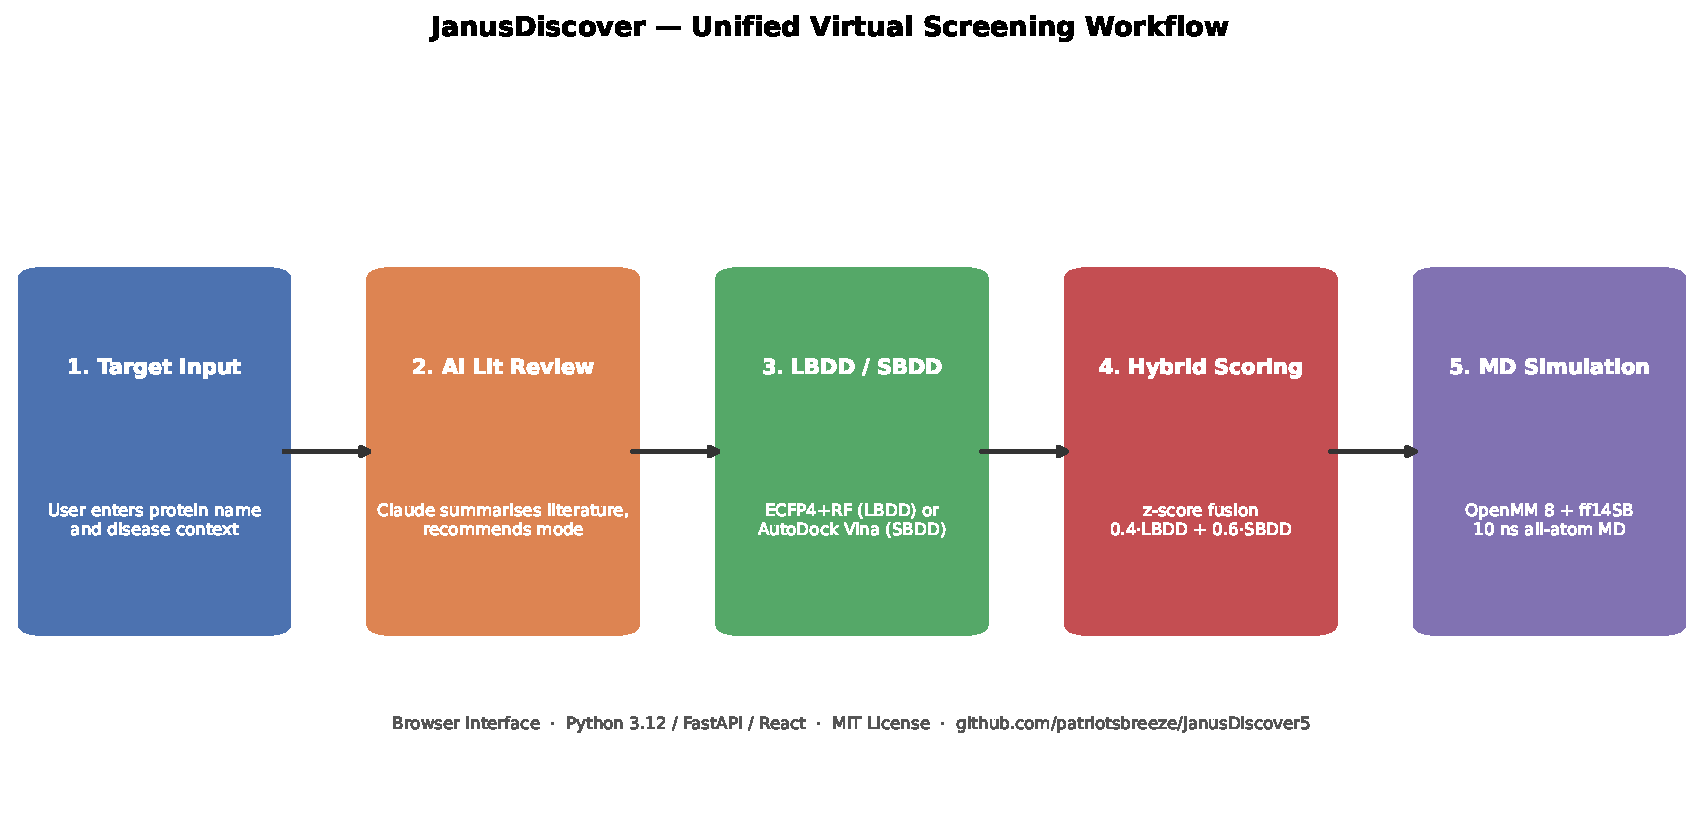
\includegraphics[width=\linewidth]{../paper/figures/workflow_overview.pdf}
\fbox{\parbox{0.9\linewidth}{\centering\vspace{2cm}
  [Figure 1: JanusDiscover workflow.\\
  Five-step pipeline: (1) target input, (2) AI literature review,
  (3) LBDD / SBDD screening, (4) hybrid consensus scoring,
  (5) optional MD validation.\\
  Replace this box with:
  \texttt{../paper/figures/workflow\_overview.pdf}]
  \vspace{2cm}}}
\caption{
  \textbf{JanusDiscover unified virtual screening workflow.}
  Starting from a protein target name, the platform automatically retrieves
  ChEMBL actives, trains an ECFP4 random forest classifier (LBDD),
  docks a ZINC-250k library with AutoDock Vina (SBDD), fuses both scores
  into a hybrid consensus, and optionally subjects the top hit to all-atom
  MD validation using OpenMM.  The entire pipeline is accessible through a
  React web interface without local software installation.
}
\label{fig:workflow}
\end{figure}

\end{document}
